\chapter{Critical Graphs on the Torus}

In this chapter we delve into the details of critical and list-critical graphs on the torus,
including Postle's approach for list-critical graphs on surfaces and Thomassen's approach
for $6$-critical graphs on the torus. 
From studying these, we develop our own, computer-aided approach
for $6$-list-critical graphs on the torus.

\section{An Overview of Postle's Approach}

Here we briefly explain Postle's approach in \cite{postlethesis} to obtain the result on the finiteness of 6-list-critical graphs in general surfaces, mentioning specially those intermediate results or definitions we will also use in our approach. The results obtained by Postle are very non-explicit in the sense that the (unspecified) constant in the size bounds for the graphs he obtains is extremely large and hence useless for our purpose of finding an explicit characterization. Nevertheless, given that our approach is primarily guided by this work we consider it of interest to provide a exposition of the main argument.

The results developed in \cite{postlethesis} in 2012 have been published successively in journal articles afterwards, often with improvements in exposition or in the strength of the result. We refer to the corresponding published article in the discussion of each particular result.

\subsection{Notation and Terminology}

Postle works mainly in a setting similar to the hypothesis of Thomassen's stronger theorem: list assignments $L$ which have list sizes of length at least $5$ for interior vertices and at least $3$ for exterior vertices with some exceptions. This setting is encapsulated in the concept of \emph{canvas}.

\begin{definition}[Canvas]
We say that $(G, S, L)$ is a \emph{canvas} if $G$ is a connected plane graph
 with outer walk $C$, $S$ is a subgraph of $C$, and $L$ is a list assignment
  such that $|L(v)| \geq 5 \, \forall v \in V(G) \setminus V(C)$ and
   $|L(v)| \geq 3 \, \forall v \in V(C) \setminus V(S)$. If $S$ is a path,
    we say $(G, S, L)$ is a \emph{path-canvas} or a \emph{wedge}. If $S = C$ and 
    $C$ is a cycle, then $(G, C, L)$ is a \emph{cycle-canvas}.
\end{definition} 



Note: in some places like \cite{fivelistcoloring2}, the term ``canvas'' is used for what Postle calls in \cite{postlethesis} ``cycle-canvas''.

We can restate Thomassen's Stronger Theorem in these terms:

\begin{theorem}
If $(G, P, L)$ is a path-canvas and $|V(P)| \leq 2$, then $G$ is $L$-colorable.
\end{theorem}

\begin{definition}[Critical canvas]
We say that a canvas $(G, S, L)$ is \emph{critical} if it is $S$-critical with respect to $L$.
\end{definition}

In the context of canvases, we usually talk of \emph{separating vertices} or \emph{separating
subgraphs} as graphs which, when removed, disconnect vertices of $S$ from other vertices in $S$.



\subsection{Variations on Thomassen's Condition}

Much of the technical work on Postle's thesis relies in a careful study of what happens if one varies the condition on \ref{thomassenstrongertheorem}. One of the most elegant (and also useful) results is the following strengthening to Thomassen's Stronger Theorem, originally conjectured by Hutchinson in \cite{hutchinson2012outerplanar}.

\begin{theorem}[Two Lists of Size Two Theorem \cite{fivelistcoloring1}]
\label{twolistsofsizetwo}
If $G$ is a plane graph with outer cycle $C$, $v_1, v_2 \in C$ and $L$ is a list assignment with $|L(v)| \geq 5$ for all $v \in V(G) \setminus V(C)$, $|L(v)| \geq 3$ for all $v \in V(C) \setminus \{v_1, v_2\}$, and $|L(v_1)| = |L(v_2)| = 2$, then $G$ is $L$-colorable. 
\end{theorem}

Or, in the language of canvases:

\begin{theorem}
If $(G, S, L)$ is a canvas with $|V(S)| = 2$ and $L(v) \geq 2$ for $v \in S$, then $G$ is $L$-colorable.
\end{theorem}

This theorem is not true when one of the two vertices has list of size $1$. In fact, Postle characterizes exactly when it fails:

\begin{definition}[Coloring Harmonica]
Let $G$ be a plane graph and $L$ a list assignment for $G$. Given an edge $uv$ and a vertex $w$ both from the outer face of $G$, we say that $(G, L)$ is a \emph{coloring harmonica from $uv$ to $w$} if either:

	\begin{itemize}
		\item $G$ is a triangle with vertex set $\{u, v, w\}$ and $L(u) = L(v) = L(w)$ with $|L(u)| = 2$, or
		\item There exists a vertex $z$ incident with the outer face of $G$ such that $uvz$ is a triangle in $G$, $L(u) = L(v) \subseteq L(z)$, $|L(u)| = |L(v)| = 2$, $|L(z)| = 3$, and the pair $(G', L')$ is a coloring harmonica from $z$ to $w$, where $G'$ is obtained by deleting \textbf{one or both} of the vertices $u$, $v$ and $L'$ is obtained from $L$ by $L'(z) = L(z) \setminus L(u)$ and $L'(x) = L(x)$ for all other vertices $z \neq x \in V(G')$.
	\end{itemize}

	Given two vertices $u, w$ in the outer face of $G$, we say $(G, L)$ is a \emph{coloring harmonica from $u$ to $w$} if there exist vertices $x, y$ incident with the outer face of $G$ such that $uxy$ is a triangle in $G$, $|L(u)| = 1$, $L(x) - L(u) = L(y) - L(u)$, $|L(x)-L(u)|=2$, and $(G', L')$ is a coloring harmonica from $xy$ to $w$, where $G'$ is obtained from $G$ by removing $u$, and $L'$ is obtained from $L$ by seting $L'(x) = L'(y) = L(x)-L(u)$ and $L'(z) = L(z)$ for every $z \in V(G') \setminus \{x, y\}$.


We say that $(G, L)$ is a coloring harmonica if it is a coloring harmonica from $uv$ to $w$ or a coloring harmonica from $u$ to $w$ for some $u, v, w$ as specified earlier.
\end{definition}

\missingfigure{harmonica}

See the example in (reference to figure) (from \cite{fivelistcoloring3}) for some clarity with respect to this mutually recursive definition. Note that the definition makes it clear that graphs which contain a coloring harmonica as a subgraph are not $L$-colorable. 

\begin{theorem}{One List of Size One and One List of Size Two Theorem \cite{fivelistcoloring3}}
Let $G$ be a plane graph with outer cycle $C$, let $p_1, p_2 \in V(C)$, and let
$L$ be a list assignment with $|L(v)| \geq 5$ for all $v \in V(G) \setminus V(C)$, $|L(v)| \geq 3$ for all
$v \in V (C) \setminus \{p_1 , p_2\}$, $|L(p_1)| \geq 1$ and $|L(p_2)| \geq 2$. Then $G$ is $L$-colorable if and only if the pair $(G, L)$ does not contain a coloring harmonica from $p_1$ to $p_2$.
\end{theorem}

Studying conditions of the sizes of the lists in the boundary in which the graph is not $L$-colorable like this one is also useful, because such conditions arise when dealing when reductions and therefore characterizing which are the critical graphs in such settings can give fruitful results.

Thomassen already studied when does the coloring of a path of length $2$ not extend:

\begin{definition}[Bellows]
	We say that a path-canvas $(G, P, L)$ with $P = p_0p_1p_2$ is a \emph{bellows} (terminology from \cite{postlethesis}) or a \emph{generalized wheel} (terminology from \cite{thomassenexponentiallymany5listcolorings}) if either:
	\begin{itemize}
		\item $G$ has no interior vertices and its edge set consists of the edges of the outer cycle plus all edges from $p_1$ to vertices of the outer cycle. In this case, we say that $(G, P, L)$ is a \emph{fan}.
		\item $G$ has one interior vertex $u$ and its edge set consists of the edges of the outer cycle plus all edges from $u$ to vertices of the outer cycle. In this case, we say that $(G, P, L)$ is a \emph{turbofan}.
		\item $G$ can be formed by gluing two smaller bellows from the edges $p_1p_2$ and $p_0p_1$ respectively. 
	\end{itemize}
\end{definition}

\missingfigure{bellows}


\begin{theorem}[\cite{thomassenexponentiallymany5listcolorings}, Theorem 3]
	If $T = (G, P, L)$ is a path-canvas with path length $2$, then $G$ is $L$-colorable unless $T$ has a bellows as a subcanvas.
\end{theorem}

Postle studies when the coloring of two paths of length $1$ does not extend. He finds the following obstruction:

\begin{definition}[Accordion]
	We say that a canvas $T = (G, P_1 \cup P_2, L)$ with $P_1, P_2$ distinct paths of length $1$ is an \emph{accordion} with \emph{ends} $P_1, P_2$ if $T$ is a bellows with $P_1 \cup P_2$ path of length $2$ or $T$ is the gluing of two smaller accordions $T_1 = (G_1, P_1 \cup U, L)$ with ends $P_1, U$ and $T_2 = (G_2, P_2 \cup U, L)$ with ends $U$, $P_2$ along a chord $U = u_1u_2$ where $|L(u_1)|, |L(u_2)| \leq 3$.
\end{definition}

The main result he obtains is that if the two paths are sufficiently far apart, then the graph contains a proportionally large accordion or a coloring harmonica as a subgraph.

\begin{theorem}[Bottleneck Theorem, loosely stated]
\label{bottlenecktheorem}
If $T = (G, P \cup P_0 , L)$ is a canvas with $P, P_0$ distinct edges of $C$ with $d(P, P_0) \geq 14$, then either there exists an $L$-coloring of $G$, or there exists a subcanvas $(G_0 , U_1 \cup U_2 , L)$ of $T$ where $d_{G_0} (U_1, U_2) = \Omega(d_G (P, P_0))$ which is an accordion or a coloring harmonica.
\end{theorem}

This result, along with coloring and structural properties of accordions and harmonicas, is often used as a technical lemma when proving the following results.

\subsection{Linear Bound on Critical Cycle-Canvases}

Postle proves the following result:

\begin{theorem}[\cite{fivelistcoloring2}]
\label{linearboundcycletheorem}
Let $G$ be a plane graph with outer cycle $C$ and $L$ a $5$-lis-assignment for $G$. Let $H$ be a minimal subgraph of $G$ such that every $L$-coloring of $C$ that extends to an $L$-coloring of $H$ also extends to an $L$-coloring of $G$. Then $H$ has at most $19|V(C)|$ vertices.
\end{theorem}

Or, equivalently stated in the language of critical canvases:

\begin{theorem}
If $(G, C, L)$ is a critical cycle-canvas, then $|V(G)| \leq 19 |V(C)|$.
\end{theorem}

The equivalence of the two statements is given by \ref{minimalsubgraphlemma}. This result is interesting in its own right because by \ref{gluinglemma}, all faces of a $T$-critical graph which do not separate vertices from $T$ are in fact critical cycle-canvases, and therefore what the result tells us is that for such graphs there is only finitely many kinds of faces that can appear for each given cycle length. This gives us a lot of information of how critical graphs look like. 

A first observation that can be made is that critical cycle-canvases (in which $C$ is indeed a simple cycle) are $2$-connected, so each face is bounded by a cycle:

\begin{lemma}
If $(G, C, L)$ is a critical cycle-canvas, then it is $2$-connected.
\end{lemma}

\begin{proof}
If $G$ is not $2$-connected, then there exist subgraphs $A, B$ such that $A \cup B = G$ with $|V(A) \cap V(B)| \leq 1$ and $|V(B) \setminus V(A)| \geq 1$. Assume $C \subseteq A$ and apply \ref{gluinglemma} to get that $B$ is $A[V(A) \cap V(B)]$-critical, contradicting \ref{thomassenstrongertheorem}.
\end{proof}

The key result in Postle's proof of the linear bound for cycles is the following theorem about the structure of critical cycle-canvases:

\begin{theorem}[Cycle Chord or Tripod Theorem]
\label{cyclechordtripodtheorem}
If $(G, C, L)$ is a critical cycle-canvas, then either

\begin{enumerate}
\item $C$ has a chord in $G$, or
\item there exists a vertex $v \in V(G) \ V(C)$ with at least three neighbors on $C$ such that at most one of the faces of $G[\{v\} \cup V(C)]$ includes a vertex or edge of $G$. 
\end{enumerate}
\end{theorem}

Using this result, Postle carefully examines what happens near the boundary cycle in order to define some quantities related to sums of lengths of faces and proves that certain inequalities with those quantites are mantained when adding tripods in critical canvases. 



\subsection{The Two Precolored Triangles Theorem}

Next, Postle proves the following theorem:

\begin{theorem}
	There exists $d$ such that the following holds.
	Let $G$ be a planar graph and $T_1, T_2$ triangles in $G$ at distance at least $d$. Let $L$ be a $5$-list-assignment of $G$. Then, every $L$-coloring of $T_1 \cup T_2$ extends to an $L$-coloring of $G$.
\end{theorem}

(Postle refers to the graphs with two precolored triangles and all other vertices with list sizes
at least $5$ as \emph{prism-canvases}, even though they are not a type of canvas).

The value of $d$ that Postle obtains is not explicitly stated, but it is on the order of $100$. However, we conjecture that $4$ or $5$ suffices.

\begin{conjecture}
\label{twotriangleconjecture}
Let $G$ be a planar graph and $T_1, T_2$ triangles in $G$ at distance at least $5$. Let $L$ be a $5$-list-assignment of $G$. Then, every $L$-coloring of $T_1 \cup T_2$ extends to an $L$-coloring of $G$.
\end{conjecture}

The argument that Postle uses to prove his result is as follows. First, he proves that one can precolor a path between the two triangles in such a way that, when deleting the path and deleting the corresponding colors from the lists of neighboring vertices, all remaining non-precolored vertices have lists of size at least $3$. The proof of this begins with the simple observation that each vertex outside a shortest path has at most $3$ neighbors inside the path. Using planarity properties, a shortest path can be found so that it can be colored in such a way that the vertices with $3$ neighbors inside the path only see two different colors from their lists.

After precoloring and deleting the path between the two triangles, a canvas $(G, P_1 \cup P_2, L)$ is obtained. If there was a precoloring of the triangles that did not extend, then the canvas contains a critical canvas, and by \ref{bottlenecktheorem} it contains a proportionally long accordion or harmonica. Postle proves that this (together with some technical details related to how the path between the triangles was chosen) implies that in the original graph there must be a long chain of separating triangles so that the graph between each separating triangle pertains to one of three very specific types, which he calls tetrahedral, octahedral or hexadecahedral bands. 

\todo{check if I defined separating triangle in introduction}

Finally, he proves that for a sufficiently long chain of this type, any precoloring of the innermost and outermost triangles extends to the whole chain. This proves the theorem, because of the following observation:

\begin{proposition}
	Let $G$ be a plane graph with $L$ a list assignment, $T_1$, $T_2$ 
	two facial triangles with $T_1$ bounding the infinite face of $G$, 
	and $T'_1$, $T'_2$ two triangles such that $T'_1$ is a separating 
	triangle between $T_1$ and $T'_2$ and $T'_2$ is a separating 
	triangle between $T'_1$ and $T_2$. Denote by $G[T'_1, T'_2]$ the 
	subgraph comprised between the two triangles $T'_1, T'_2$.  
	If there exists some $L$-coloring of $T_1 \cup T_2$ that does not 
	extend to $G$, then there exists some $L$-coloring of $T'_1 \cup T'_2$ 
	that does not extend to $G[T'_1, T'_2]$.
\end{proposition}

\begin{proof}
	By \ref{thomassenstrongertheorem}, the coloring on $T_1$ extends to 
	$G[T_1, T'_1]$ and the coloring on $T_2$ extends to $G[T'_2, T_2]$. 
	The coloring of $T'_1 \cup T'_2$ given by this extensions can not 
	extend to $G[T'_1, T'_2]$ by the assumption that the original coloring 
	of $T_1 \cup T_2$ did not extend to $G$.
\end{proof}

\subsection{Cylinder-Canvases and Hyperbolic Families}

Finally, Postle generalizes the previous setting of critical prism-canvases to \emph{critical cylinder-
canvases}, where a cylinder-canvas is like a prism-canvas but the precolored cycles can have length
greater than $3$. It generalizes Theorem \ref{twoprecoloredtrianglestheorem} by showing that for
every pair of cycle lengths, there exists a distance $d$ (depending logarithmically on the cycle sizes)
so that all critical cylinder-canvases have the cycles at distance at most $d$. It also generalizes
Theorem \ref{linearboundcycletheorem} by showing that critical cylinder-canvases have a bound
on their size linear in the sum of the cycle lengths.

Then, he defines \emph{hyperbolic families}: families of graphs embedded in surfaces which have
certain properties related to having planar graphs resulting from performing \emph{excisions} in
the surface always having bounded size. We do not delve into the details because the topological
arguments for the general case are not of interest for us, but we will explain some similar
operations on the torus in the section explaining our approach. 

The idea here is that the linear bounds on the cycle-canvases and the cylinder-canvases make the 
$6$-list-critical graphs on the torus be an hyperbolic family. Then, the result we want about
the finiteness of $6$-list-critical graphs is proven for the more general setting of hyperbolic
families. In fact, it is proven that the number of vertices of such is bounded linearly by the genus 
of the surface.

The general setting of hyperbolic surfaces allows Postle to prove more properties and bounds of
$6$-list-critical graphs on the torus, such as:

\begin{theorem}
\label{edgewidththeorem}
Let $G$ be a graph 2-cell-embedded in a surface $\Sigma$ and let $L$ be a $5$-list-assignment.
If $ew(G) \geq O(\log g(\Sigma))$, then $G$ is $L$-colorable. 

\end{theorem}





\section{Critical Graphs on the Torus for (usual) Vertex Coloring}

In this section we discuss the result from Thomassen in \cite{thomassentorus} that characterizes the critical graphs for $5$-coloring (not $5$-list-coloring) on the torus.

\subsection{The Critical Graphs}

\begin{theorem}[\cite{thomassentorus}]
	\label{thomassentorustheorem}
	A graph $G$ embeddable on the torus is $5$-colorable if and only if 
	it does not contain the following subgraphs:
	\begin{itemize}
		\item $K_6$.
		\item $C_3 + C_5$.
		\item $K_2 + H_7$, where $H_7$ is a $7$-vertex graph known as the \emph{Moser spindle}.
		\item $T_{11}$, where $T_{11}$ is a triangulation of the torus with $11$ vertices.
	\end{itemize}
	Where $+$ denotes the join of two graphs: their disjoint union with 
	all pairs of vertices from different graphs joined by edges.
\end{theorem} 


\begin{figure}
\centering
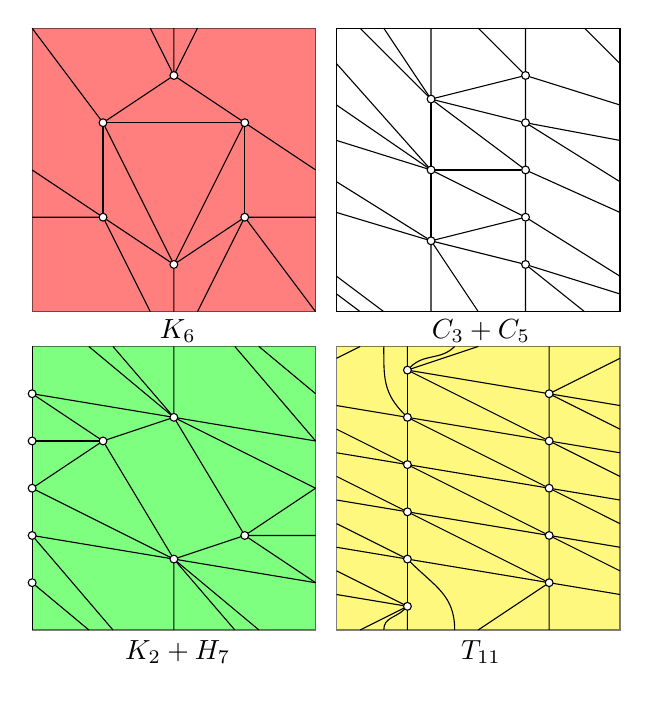
\begin{tikzpicture}[main/.style = {draw, circle, fill=white}]

\begin{scope}[scale=0.3, every node/.append style={transform shape}]]
\draw[draw=black, fill=red, opacity=0.5] (0, 0) rectangle (12, 12);




\node[main] (A1) at (6, 10) {};
\node[main] (A2) at (3, 4) {};
\node[main] (A3) at (9, 4) {};

\node[main] (B1) at (6, 2){};
\node[main] (B2) at (9, 8) {};
\node[main] (B3) at (3, 8) {};


\draw (A1) -- (B2);
\draw (B2) -- (A3);
\draw (A3) -- (B1);
\draw (B1) -- (A2);
\draw (A2) -- (B3);
\draw (B3) -- (A1);

\draw (A1) -- (6, 12);
\draw (6, 0) -- (B1);
%\draw (A2) -- (0, 0);
%\draw (12, 12) -- (B2);
\draw (A3) -- (12, 0);
\draw (0, 12) -- (B3);

\draw (A2) -- (0, 6);
\draw (12, 6) -- (B2);

\draw (B1) -- (B2);
\draw (B2) -- (B3);
\draw (B3) -- (B1);

\draw (A2) -- (0, 4);
\draw (12, 4) -- (A3);
\draw (A2) -- (5, 0);
\draw (5, 12) -- (A1);
\draw (A3) -- (7, 0);
\draw (7, 12) -- (A1);


\end{scope}

\begin{scope}[xshift=110, scale=0.3, every node/.append style={transform shape}]]
\draw[draw=black] (0, 0) rectangle (12, 12);




\node[main] (A1) at (4, 9) {};
\node[main] (A2) at (4, 6) {};
\node[main] (A3) at (4, 3) {};



\node[main] (B1) at (8, 10){};
\node[main] (B2) at (8, 8) {};
\node[main] (B3) at (8, 6) {};
\node[main] (B4) at (8, 4) {};
\node[main] (B5) at (8, 2) {};


\draw (4, 12) -- (A1);
\draw (A1) -- (A2);
\draw (A2) -- (A3);
\draw (A3) -- (4, 0);

\draw (8, 12) -- (B1);
\draw (B1) -- (B2);
\draw (B2) -- (B3);
\draw (B3) -- (B4);
\draw (B4) -- (B5);
\draw (B5) -- (8, 0);

\draw (A1) -- (B1);
\draw (A1) -- (B2);
\draw (A1) -- (B3);
\draw (A1) -- (2, 12);
\draw (2, 0) -- (0, 1.5);
\draw (12, 1.5) -- (B4);
\draw (A1) -- (1, 12);
\draw (1, 0) -- (0, 0.75);
\draw (12, 0.75) -- (B5);

\draw (A2) -- (B3);
\draw (A2) -- (B4);
\draw (A2) -- (0, 10.5);
\draw (12, 10.5) -- (10.5, 12);
\draw (10.5, 0) -- (B5);
\draw (A2) -- (0, 8.75);
\draw (12, 8.75) -- (B1);
\draw (A2) -- (0, 7.25);
\draw (12, 7.25) -- (B2);


\draw (A3) -- (B4);
\draw (A3) -- (B5);
\draw (A3) -- (6, 0);
\draw (6, 12) -- (B1);
\draw (A3) -- (0, 5.5);
\draw (12, 5.5) -- (B2);
\draw (A3) -- (0, 4.2);
\draw (12, 4.2) -- (B3);

\end{scope}


\begin{scope}[yshift=-115, scale=0.3, every node/.append style={transform shape}]]
\draw[draw=black, fill=green, opacity=0.5] (0, 0) rectangle (12, 12);




\node[main] (A1) at (0, 8) {};
\node[main] (A2) at (0, 10) {};
\node[main] (A3) at (0, 2) {};
\node[main] (A4) at (0, 4) {};
\node[main] (A5) at (0, 6) {};

\coordinate[] (A1c) at (12, 8) {};
\coordinate[] (A2c) at (12, 10) {};
\coordinate[] (A3c) at (12, 2) {};
\coordinate[] (A4c) at (12, 4) {};
\coordinate[] (A5c) at (12, 6) {};

\node[main] (H1) at (3, 8) {};
\node[main] (H2) at (9, 4) {};

\node[main] (K1) at (6, 9) {};
\node[main] (K2) at (6, 3) {};




\draw (A1) -- (A2);
\draw (A2) -- (0, 12);
\draw (0, 0) -- (A3);
\draw (A3) -- (A4);
\draw (A4) -- (A5);
\draw (A5) -- (A1);

\draw (H1) -- (A1);
\draw (H1) -- (A2);
\draw (H1) -- (A5);

\draw (H2) -- (A3c);
\draw (H2) -- (A4c);
\draw (H2) -- (A5c);

\draw (K1) -- (A2);
\draw (K1) -- (A1c);
\draw (K1) -- (A5c);
\draw (K1) -- (H1);
\draw (K1) -- (H2);
\draw (K1) -- (3.42, 12);
\draw (3.42, 0) -- (A4);
\draw (K1) -- (2.4, 12);
\draw (2.4, 0) -- (A3);

\draw (K2) -- (A5);
\draw (K2) -- (A4);
\draw (K2) -- (A3c);
\draw (K2) -- (H1);
\draw (K2) -- (H2);
\draw (K2) -- (12-3.42, 0);
\draw (12-3.42, 12) -- (A1c);
\draw (K2) -- (12-2.4, 0);
\draw (12-2.4, 12) -- (A2c);


\draw (K1) -- (6, 12);
\draw (6, 0) -- (K2);
\end{scope}

\begin{scope}[xshift=110, yshift=-115, scale=0.3, every node/.append style={transform shape}]]
\draw[draw=black, fill=yellow, opacity=0.5] (0, 0) rectangle (12, 12);




\node[main] (A0) at (3, 11) {};
\node[main] (A1) at (3, 9) {};
\node[main] (A2) at (3, 7) {};
\node[main] (A3) at (3, 5) {};
\node[main] (A4) at (3, 3) {};
\node[main] (A5) at (3, 1) {};

\node[main] (B0) at (9, 10) {};
\node[main] (B1) at (9, 8) {};
\node[main] (B2) at (9, 6) {};
\node[main] (B3) at (9, 4) {};
\node[main] (B4) at (9, 2) {};

\draw (A0) -- (A1);
\draw (A1) -- (A2);
\draw (A2) -- (A3);
\draw (A3) -- (A4);
\draw (A4) -- (A5);

\draw (B0) -- (B1);
\draw (B1) -- (B2);
\draw (B2) -- (B3);
\draw (B3) -- (B4);

\draw (A0) -- (B0);
\draw (A0) -- (B1);
\draw (A1) -- (B1);
\draw (A1) -- (B2);
\draw (A2) -- (B2);
\draw (A2) -- (B3);
\draw (A3) -- (B3);
\draw (A3) -- (B4);
\draw (A4) -- (B4);

\draw (B0) -- (12, 9.5);
\draw (0, 9.5) -- (A1);
\draw (B0) -- (12, 8.5);
\draw (0, 8.5) -- (A2);
\draw (B1) -- (12, 7.5);
\draw (0, 7.5) -- (A2);
\draw (B1) -- (12, 6.5);
\draw (0, 6.5) -- (A3);
\draw (B2) -- (12, 5.5);
\draw (0, 5.5) -- (A3);
\draw (B2) -- (12, 4.5);
\draw (0, 4.5) -- (A4);
\draw (B3) -- (12, 3.5);
\draw (0, 3.5) -- (A4);
\draw (B3) -- (12, 2.5);
\draw (0, 2.5) -- (A5);
\draw (B4) -- (12, 1.5);
\draw (0, 1.5) -- (A5);

\draw (A4) to [out=-45, in=90, looseness=1.1] (5, 0);

\draw (5, 12) to [out = -135, in = 45, looseness=1.05] (A0);

\draw (B4) -- (6, 0);
\draw (6, 12) -- (A0);
\draw (B4) -- (9, 0);
\draw (9, 12) -- (B0);

\draw (A5) -- (3, 0);
\draw (3, 12) -- (A0);
\draw (A5) to [out=-135, in = 90, looseness=1.1] (2, 0);
\draw (2, 12) to [out=-90, in =135, looseness=1.1] (A1);
\draw (A5) -- (1, 0);
\draw (1, 12) -- (0, 11.5);
\draw (12, 11.5) -- (B0);

\end{scope}

\node[] at (1.85, -0.25) {$K_6$};
\node[] at (5.70, -0.25) {$C_3+C_5$};
\node[] at (1.85, -4.32) {$K_2+H_7$};
\node[] at (5.70, -4.32) {$T_{11}$};
\end{tikzpicture}
\caption{$6$-critical graphs embedded on the torus.}
\end{figure}

If a graph is not $5$-colorable, it is not $5$-list-colorable, so all graphs 
that contain any of the above subgraphs are not $5$-list-colorable. 
We conjecture that this characterizes the $5$-list-colorable graphs on the torus too:

\begin{conjecture}
\label{torusconjecture}
A graph $G$ embeddable on the torus is $5$-list-colorable if and only if 
it does not contain the following subgraphs: $K_6$, $C_3 + C_5$, $K_2 + H_7$, $T_{11}$.
\end{conjecture}

This means that those are the minimal $6$-list-critical graphs on the torus. Note 
that there may be additional $6$-list-critical graphs embeddable on the torus, but what we are conjecturing is that they all 
contain those subgraphs. For example:

\begin{observation}
$K_7$ is $6$-list-critical.
\end{observation}

\begin{proof}
Consider the following $5$-list-assignment for $K_7$: $L(v_1) = L(v_2) = L(v_3) = L(v_4) = L(v_5) = \{1, 2, 3, 4, 5\}$, 
$L(v_6) = L(v_7) = \{1, 2, 3, 4, 6\}$. $K_7$ is not $L$-colorable, since there are only $6$ available colors. 
But any subgraph is $L$-colorable. Let's give a coloring $\phi$ for $K_7 \setminus v_iv_j$. If $i, j \leq 5$, 
then setting $\phi(v_i) = \phi(v_j) = 5$ and $\phi(v_7) = 6$ leaves $4$ vertices to be colored with $4$ colors. 
If $i \leq 5$ and $j \geq 6$, then setting $\phi(v_i) = \phi(v_j) = 1$, $\phi(v_{13-j}) = 6$ leaves $4$ vertices 
to be colored with $4$ colors. If $\{i, j\} = \{6, 7\}$, then $\phi(v_i) = \phi(v_j) = 6$ leaves $5$ vertices 
to be colored with $5$ colors.

Hence, $K_7$ is $L$-critical for a $5$-list-assignment $L$, and is therefore $6$-list-critical.
\end{proof}

\subsection{An Overview of Thomassen's Approach}

Thomassen's article where he characterizes the graphs on the torus (\cite{thomassentorus}) predates 
his result on finitely many $6$-critical graphs for all surfaces (\cite{thomassenfixedsurface}). 
For the characterization of $6$-critical graphs on the torus, he only uses elementary, relatively 
straighforward arguments that work on specifically in the torus. We briefly summarize his 
approach here in order to discuss which arguments can be reused for the list-coloring case. 

First, Thomassen considers the case when the minimum degree is at least $6$. 

\begin{proposition}
If a graph $G$ embedded on the torus has $\delta(G) \geq 6$, then:

\begin{enumerate}
	\item $G$ is $6$-regular.
	\item $G$ is a triangulation of the torus.
\end{enumerate}
\end{proposition}

\begin{proof}
We apply Euler's formula: let $V, E, F$ be the number of vertices, edges and faces in the embedding, respectively. 
We have that $\delta(G) \geq 6 \implies V \leq \frac{1}{3} E$ with equality iff $G$ is $6$-regular, and $F \leq \frac{2}{3}E$ 
with equality iff $G$ is a triangulation. Then $0 = V - E + F \leq \frac{1}{3}E - E + \frac{2}{3}E = 0$, so we have equality on both inequalities.
\end{proof}

Using the proposition above, Thomassen then proves the following:

\begin{proposition}[3.2 in \cite{thomassentorus}]
Let $G$ be a $6$-regular graph on the torus. If $G$ contains a vertex $v$, such that $\{v\} \cup N(v)$ induces a nonplanar graph, then $G = K_7$ or $G$ is obtained from $K_8$ or $K_9$ by deleting the edges of a $1$-regular or $2$-regular subgraph.
\end{proposition}

The study of $6$-regular graphs on the torus without vertices whose neighborhood induces a nonplanar graph was already done by Thomassen in his previous paper \cite{thomassentilings}, in the context of finding all tilings of the torus in order to prove a conjecture by Babai about vertex-transitive graphs. 

He obtains the following result:

\begin{theorem}
Let $G$ be a graph embedded on the torus with $\delta(G) \geq 6$. Then $G$ is $5$-colorable 
unless $G = K_7$ or $G = T_{11}$.
\end{theorem}

This part of the argument is the one that can be generalized to list coloring, but it is not
useful to our approach, so we don't delve into the details. 

Let us now describe Thomassen's argument for 
general graphs.

He assumes a minimum counterexample $G_0$ to \ref{thomassentorustheorem} (the counterexample has
minimum number of vertices, maximum number of edges restricted to that, and some other assumptions 
about details we will not discuss here). By the previous result, 
there must be a vertex $v_0 \in V(G_0)$ with degree $\leq 5$, and the degree of $v_0$ is in 
fact equal to $5$ by minimality of the counterexample. 

Consider two vertices $x, y \in N(v_0)$ which are not adjacent (if all the vertices of 
$N(v_0)$ were adjacent, then $G_0$ would contain $K_6$, a contradiction). Let $G_{xy}$ be 
the graph obtained from $G_0 \setminus v_0$ by identifying the vertices $x$ and $y$. 
$G_{xy}$ can be embedded in the torus by modifying the embedding of $G_0$. If $G_{xy}$ 
were $5$-colorable, then we would have a $5$-coloring of $G_0$ by assigning the same color 
to $x$ and $y$ and coloring $v_0$ with a color not appearing in its $5$ neighbors. 
Hence, $G_{xy}$ is not $5$-colorable and by minimality of our counterexample it 
contains $K_6$, $C_3 + C_5$, $K_2 + H_7$ or $T_{11}$.

The above argument works for all pairs $x, y$ of non-adjacent vertices in $N(v_0)$, so potentially 
we can have many different obstructions for each of the corresponding $G_{xy}$ subgraphs. 
But we can prove that, by minimality, there can not be much else in $G_0$ apart from these
obstructions arising from all the $G_{xy}$ subgraphs. More precisely:  

\begin{proposition}
	\label{g0proposition}
	For any non-adjacent $x, y \in N(v_0)$, let $G'_{xy}$ a copy of 
	$K_6$, $C_3 + C_5$, $K_2 + H_7$ or $T_{11}$ in $G_{xy}$, and let $G''_{xy}$ be the induced
	subgraph of $G_{xy}$ by the vertex set of $G'_{xy}$. Then $G_0$ consists of $v_0$, $N(v_0)$, 
	the edges between vertices of $\{v_0\} \cup N(v_0)$, and the union over all non-adjacent 
	$x, y \in N(v_0)$ of the graph obtained from $G''_{xy}$ by splitting the contracted vertex
	into $x$ and $y$.  
\end{proposition}

\begin{proof}
We will prove that the graph described above, which is a subgraph of $G_0$, is not $5$-colorable. 
This means, by the assumptions of minimality of vertices and maximality of edges, that $G_0$ is
in fact equal to that subgraph. 

If the subgraph had a $5$-coloring, then two non-adjacent vertices $x, y$ of $N(v_0)$ would 
have the same color. But by then identifying the two vertices we can get a $5$-coloring 
of $G''_{xy}$, which contains the non-$5$-colorable subgraph $G'_{xy}$, contradiction.

\end{proof}

Note that, since the maximum number of vertices in a critical graph is $11$, this means that
$G_0$ has at most $(11 - 1) \cdot \binom{5}{2} + 6 = 106$ vertices, and hence what remains
is a finite problem.

Thomassen uses some more arguments to narrow down the remaining possibilities for $G_0$, but
we can already see an important point of failure of this argument for list-coloring: in the 
proof of \ref{g0proposition}, it is used that a necessary and sufficient condition for a coloring
of $G_0 \setminus v_0$ to extend to $v_0$ is that two neighbors of $v_0$ have the same color.
In list coloring, this condition is not necessary. So we cannot conclude that the minimum 
counterexample is the union of the graphs induced by the obstructions in $G_{xy}$ and the 
argument breaks down here. 











\section{Our Approach}

The bounds on the size of $6$-list-critical graphs on the torus given by Postle's approach are 
way too large to be of any use to us in our search of the explicit list for the torus. However, 
we can take inspiration in his approach and in particular in how it was useful to carefully study
critical canvases. The key modification is that, instead of proving abstract bounds for sizes
of critical canvases as in Theorem \ref{linearboundcycletheorem}, we will be working with the 
explicit, full list of critical canvases of a certain type and size. 

In order to obtain those canvases, we will be using computer search, so this will be a 
computer-aided proof, like the Four Color Theorem's (but using very different techniques). The 
reason we consider it feasible to perform this search is that results like 
Theorem \ref{cyclechordortripodtheorem} give very structured descriptions of 
critical canvases - so we don't face enormously huge space of searching among
all the planar graphs with a given size bound, but instead have a much more restricted
search space. 

Once we have generated some critical canvases, our idea is to take advantage of them in a way 
similar to Postle's approach - but this time, 
since we will work with the explicit canvases instead of loose bounds, the hope is that we
can use them to obtain also the explicit list of $6$-list-critical graphs. 

Since the torus is not a complicated surface, there are simple manipulations 
that relate $6$-list-critical graphs on the torus with critical prism-canvases
 and cycle-canvases, as we will see now. 

\subsection{Cutting Through a Non-Contractible Cycle}

Consider the torus $S_1$. If one cuts through non-contractible curve
\todo{check if this is the appropiate term} 
one obtains a cylinder,
which can then be projected to the plane. 

We can do this to get planar graphs from graphs $2$-cell-embedded on the torus: we can cut 
through a non-contractible cycle, duplicate the vertices on the cycle so they appear on both
sides of the resulting cylinder, and then project this cylinder into the plane. See Figure \ref{fig:k6criticalprismcanvas} for an example with $K_6$, one of the $6$-critical graphs
embedded on the torus. 

\begin{figure}
\label{fig:k6criticalprismcanvas}
\centering
\begin{tikzpicture}[main/.style = {draw, circle, fill=white}]

\begin{scope}[scale=0.3, every node/.append style={transform shape}]]
\input{figures/k6_cuttingthroughcycle.tex}
\end{scope}

\node () at (4.5, 1.75) {$\implies$};

\begin{scope}[xshift=210,yshift=35, scale=0.45, every node/.append style={transform shape}]
\VertexI[x=-5, y=-2.5] {A1}
\VertexI[x=5,  y=-2.5] {A2}
\VertexI[x=0,  y=5] {A3}

\VertexV[x=-3, y=-1.5] {B1}
\VertexV[x=3,  y=-1.5] {B2}
\VertexV[x=0,  y=3] {B3}

\VertexI[x=-1, y=0] {C1}
\VertexI[x=1,  y=0] {C2}
\VertexI[x=0,  y=1.5] {C3}

\Edge(A1)(A2)
\Edge(A2)(A3)
\Edge(A3)(A1)

\Edge(C1)(C2)
\Edge(C2)(C3)
\Edge(C3)(C1)

\Edge(A1)(B3)
\Edge(A2)(B3)
\Edge(A3)(B3)
\Edge(A2)(B1)

\Edge(B1)(B3)
\Edge(B2)(B3)
\Edge(B1)(B2)

\Edge(B1)(C3)
\Edge(B1)(C1)
\Edge(B2)(C1)
\Edge(B2)(C2)
\Edge(B2)(C3)


\end{scope}
\end{tikzpicture}
\caption{Cutting $K_6$ into a critical prism-canvas.}
\end{figure}

The reason why this is useful to us is the following observation:

\begin{observation}
Let $G$ be a graph embedded on the torus, let $G'$ be a graph obtained by 
this procedure from $G$, let $C_1, C_2$ be the two cycles of $G;$ corresponding to the
non-contractible cycle $C$ of $G$ we cut through, let $L$ be a list assignment for $G$ and let
$L'$ be the corresponding list assignment for $G'$ (with the same lists for all vertices,
duplicated for $C_1$ and $C_2$).

If $G$ is $L$-critical, then $G'$ is $(C_1 \cup C_2)$-critical with respect to the
list assignment $L'$.
\end{observation}

\begin{proof}
Consider a subgraph $(C_1 \cup C_2) \subseteq H' \subset G'$ and
the corresponding subgraph $C \subseteq H \subset G$. 
By $L$-criticality of $G$, $H$ is $L$-colorable with a coloring $\phi$.
Consider the corresponding coloring $\phi'$ of $H'$.
 Then, $\phi'_{\restriction_{C_1 \cup C_2}}$
is a coloring of $(C_1 \cup C_2)$ which extends to $H'$ but not to $G'$, since if it extended
to $G'$ we would have a $L'$-coloring of $G'$ in which the corresponding vertices of $C_1$ and
$C_2$ have the same colors and therefore we would be able to retrieve an $L$-coloring of $G$.
\end{proof}

This, together with Theorem \ref{twotriangletheorem}, already places a restriction on how the
$6$-list-critical graphs on the torus can be: if the graph has a non-contractible triangle, then
it must also have a not too large non-contractible cycle not homotopically equivalent to 
the non-contractible triangle, since if the two precolored triangles are at distance $d$ in the
resulting planar graph, then there is such a non-contractible cycle of length $\leq d+1$ in the
original graph. 

An interesting implication is also that we can do the process backwards: if we have a critical 
prism-canvas, we can ``fuse the two triangles'' to get a graph on the torus which is 
\emph{possibly} $6$-list-critical.   

\subsection{Cutting Across Two Non-Contractible Cycles}

Instead of just cutting through one non-contractible cycle to get a cylinder and project it to the
plane, we can cut through two non-homotopically-equivalent non-contractible cycles to get the 
plane, as in Figure \ref{fig:twocycles_illustration}. This can be thought also as first cutting 
through a cycle to get a cylinder, and then cutting through the cylinder to get the plane. 

\begin{figure}
\label{fig:twocycles_illustration}
\centering
\begin{tikzpicture}[main/.style = {draw, circle, fill=white}]

\begin{scope}[scale=0.3, every node/.append style={transform shape}]
\draw[draw=black] (0, 0) rectangle (12, 12);

\draw[fill=blue, opacity=0.3] (6, 6) rectangle (12, 12);
\draw[fill=yellow, opacity=0.3] (6, 0) rectangle (12, 6);
\draw[fill=green, opacity=0.3] (0, 0) rectangle (6, 6);
\draw[fill=red, opacity=0.3] (0, 6) rectangle (6, 12);

\node[] (A1) at (3, 6) {};
\node[] (A2) at (6, 6) {};
\node[] (A3) at (9, 6) {};

\node[] (B1) at (6, 9){};
\node[] (B3) at (6, 3) {};

\draw[densely dashed, thick] (A1) -- (A2);
\draw[densely dotted, thick] (A2) -- (A3);
\draw[ultra thick] (B1) -- (A2);
\draw[loosely dotted, thick] (A2) -- (B3);
\draw[dashdotdotted, ultra thick] (A1) -- (0, 6);
\draw[dashdotdotted, ultra thick] (12, 6) -- (A3);
\draw[loosely dashed, thick] (B1) -- (6, 12);
\draw[loosely dashed, thick] (6, 0) -- (B3);




\end{scope}

\node () at (4.5, 1.75) {$\implies$};

\begin{scope}[xshift=200,yshift=50, scale=0.45, every node/.append style={transform shape}]
\VertexInv[x=0, y=4]{A1}
\VertexInv[x=2, y=3]{B1}
\VertexInv[x=3, y=2]{C1}
\VertexInv[x=4, y=0]{A2}
\VertexInv[x=3, y=-2]{E1}
\VertexInv[x=2, y=-3]{D1}
\VertexInv[x=0, y=-4]{A3}
\VertexInv[x=-2, y=-3]{C2}
\VertexInv[x=-3, y=-2]{B2}
\VertexInv[x=-4, y=0]{A4}
\VertexInv[x=-3, y=2]{D2}
\VertexInv[x=-2, y=3]{E2}

\VertexInv[x=2.5, y=2.5]{X1}
\VertexInv[x=2.5, y=-2.5]{X2}
\VertexInv[x=-2.5, y=-2.5]{X3}
\VertexInv[x=-2.5, y=2.5]{X4}


\draw [dotted, thick] (A1) -- (B1);
\draw [dashdotdotted, ultra thick] (B1) -- (C1);
\draw [densely dashed, thick] (C1) -- (A2);
\draw [loosely dotted, thick] (A2) -- (E1);
\draw [loosely dashed, thick] (E1) -- (D1);
\draw [ultra thick] (D1) -- (A3);
\draw [densely dashed, thick] (A3) -- (C2);
\draw [dashdotted, ultra thick] (C2) -- (B2);
\draw [densely dotted, thick] (B2) -- (A4);
\draw [ultra thick] (A4) -- (D2);
\draw [loosely dashed, thick] (D2) -- (E2);
\draw [loosely dotted, thick] (E2) -- (A1);

\fill[yellow, opacity=0.3] (-2.5, 2.5) -- (2.5,2.5) -- (0,0) -- (-2.5,2.5);
\fill[yellow, opacity=0.3] (X4) -- (E2) -- (0,4) -- (X4);
\fill[yellow, opacity=0.3] (X1) -- (B1) -- (0,4) -- (X1);
\fill[yellow, opacity=0.3] (-2.5,2.5) -- (2.5,2.5) -- (0,4) -- (-2.5,2.5);

\fill[green, opacity=0.3] (2.5, 2.5) -- (2.5,-2.5) -- (0,0) -- (2.5,2.5);
\fill[green, opacity=0.3] (X1) -- (C1) -- (4,0) -- (X1);
\fill[green, opacity=0.3] (X2) -- (E1) -- (4,0) -- (X2);
\fill[green, opacity=0.3] (2.5,2.5) -- (2.5,-2.5) -- (4,0) -- (2.5,2.5);

\fill[red, opacity=0.3] (-2.5, -2.5) -- (2.5,-2.5) -- (0,0) -- (-2.5,-2.5);
\fill[red, opacity=0.3] (X2) -- (D1) -- (0,-4) -- (X2);
\fill[red, opacity=0.3] (X3) -- (C2) -- (0,-4) -- (X3);
\fill[red, opacity=0.3] (-2.5,-2.5) -- (2.5,-2.5) -- (0,-4) -- (-2.5,-2.5);

\fill[blue, opacity=0.3] (-2.5, -2.5) -- (-2.5,2.5) -- (0,0) -- (-2.5,-2.5);
\fill[blue, opacity=0.3] (X3) -- (B2) -- (-4,0) -- (X3);
\fill[blue, opacity=0.3] (X4) -- (D2) -- (-4,0) -- (X4);
\fill[blue, opacity=0.3] (-2.5,-2.5) -- (-2.5,2.5) -- (-4,0) -- (-2.5,-2.5);


\end{scope}




\end{tikzpicture}
\caption{Cutting the torus into the plane.}
\end{figure}

The idea here is again that we can use this to get critical planar graphs from critical graphs
on the torus, but now we get a cycle-canvas instead of a prism-canvas. See Figure \ref{fig:k6_cyclecanvas} for an example again with $K_6$.

\begin{figure}
\label{fig:k6_cyclecanvas}
\centering
\begin{tikzpicture}[main/.style = {draw, circle, fill=white}]

\begin{scope}[scale=0.3, every node/.append style={transform shape}]
\input{figures/k6_cuttingthroughtwocycles.tex}
\end{scope}

\node () at (4.5, 1.75) {$\implies$};

\begin{scope}[xshift=200,yshift=50, scale=0.45, every node/.append style={transform shape}]
\VertexI[x=0, y=4]{A1}
\VertexI[x=2, y=3]{B1}
\VertexI[x=3, y=2]{C1}
\VertexI[x=4, y=0]{A2}
\VertexI[x=3, y=-2]{E1}
\VertexI[x=2, y=-3]{D1}
\VertexI[x=0, y=-4]{A3}
\VertexI[x=-2, y=-3]{C2}
\VertexI[x=-3, y=-2]{B2}
\VertexI[x=-4, y=0]{A4}
\VertexI[x=-3, y=2]{D2}
\VertexI[x=-2, y=3]{E2}

\VertexV[x=-2, y=0]{F}

\Edge(A1)(B1)
\Edge(B1)(C1)
\Edge(C1)(A2)
\Edge(A2)(E1)
\Edge(E1)(D1)
\Edge(D1)(A3)
\Edge(A3)(C2)
\Edge(C2)(B2)
\Edge(B2)(A4)
\Edge(A4)(D2)
\Edge(D2)(E2)
\Edge(E2)(A1)

\Edge(E2)(B1)
\Edge(B1)(D1)
\Edge(C1)(E1)
\Edge(D1)(C2)
\Edge(F)(C2)
\Edge(F)(B2)
\Edge(F)(A4)
\Edge(F)(D2)
\Edge(F)(E2)

\end{scope}
\end{tikzpicture}
\caption{Cutting $K_6$ into a critical cycle-canvas.}
\end{figure}

\begin{observation}
Let $G$ be a $L$-critical graph embedded on the torus with $L$ a $5$-list-assignment,
and let $G'$ be the corresponding planar graph resulting from this procedure with outer face $C$
corresponding to the two cycles we cut through. Then $(G', C, L)$ is a critical cycle-canvas.
\end{observation}

\begin{proof}
Similar argument to the previous observation.
\end{proof}

If the cycles we cut through have lengths $a$ and $b$, the resulting cycle-canvas has cycle length
$2(a+b)$. This gives a bound for the sizes of $6$-list-critical graphs in terms of the sizes of 
their non-contractible cycles via Theorem \ref{linearboundcycletheorem}. However, here the more
interesting idea is the possibility of running the process backwards: that is, of generating
candidates for $6$-list-critical graphs from critical cycle-canvases. 
That is because, as we will see, we have a procedure for the generation of all critical
cycle-canvases by computer. 


\subsection{Our Plan for Graphs With a Non-Contractible Triangle}



Using the above two constructions, we can already devise a plan for finding all $6$-list-critical 
graphs on the torus which have at least one non-contractible triangle.

\begin{enumerate}
	\item Generate all critical cycle-canvases with small cycle sizes (ideally at least up to 
	size $14$ or, better yet, $16$). Also, depending on the approach followed in the next step, it will also be 
	necessary to generate small critical path-canvases or other kinds of critical graphs. 
	\item Prove Conjecture \ref{twotriangleconjecture}. Here, we will try to take advantage
	of the computer-generated graphs in order to obtain the tightest possible bound instead of
	Postle's loose bound.
	\item By cutting through the non-contractible triangle of any $6$-list-critical graph, we
	obtain a critical prism-canvas, and therefore we can reconstruct all possible candidates
	from either the list of all critical prism-canvases (if we obtained such a list from the
	previous step) or a list of all critical cycle-canvases of size $\leq 16$ (by cutting 
	across the non-contractible triangle and the other non-contractible cycle of length 
	$\leq 5$ corresponding to the shortest path between the two precolored triangles in the
	prism-canvas).
\end{enumerate}

This plan only works for $6$-list-critical graphs with edge-width $3$, which is the case for 
the $6$-critical graphs for the previous section. We don't expect to have additional $6$-list-
critical graphs with larger edge-width, especially given (REF POSTLE RESULT EDGEWIDTH), so our
hope would be to find an argument independent of this plan to prove that any $6$-list-critical
graph on the torus must have a non-contractible triangle. 

\todo{check that I defined edge-width and given the result of Postle for ew}

\todo{references for chapters}

The rest of this thesis will be dedicated to describe how to carry out this plan. 
For the first step, we will explain how to perform the computer generation of such critical graphs
in Chapters 3 and 4. Chapter 3 will be about the computer representation of the canvases 	
and the algorithms used for the generation of candidates to be critical canvases, while 
Chapter 4 will be on how to test that such candidates are indeed critical. The techniques 
explained in Chapters 3 and 4 will be applicable not only to cycle-canvases but also to other
types of canvases or graphs with prescribed list sizes more generally. 

For the second step, in Chapter 5 we will explain different approaches to proving Conjecture 
\ref{twotriangleconjecture} using the computer-generated graphs. As of the writing of this thesis,
we have not been able find a proof of this results, because there have been computational and
conceptual obstacles in the approaches we have tried. We will also discuss those setbacks.

Finally, in Chapter 6 we will summarize the computational results obtained by the implementation
of the ideas discussed in the previous chapters and we will expose the partial results we 
have been able to obtain with respect to the third step of the plan. 



 
